\chapter{Contour plots}
\label{app:references_end_chapters}

\graphicspath{{appendix_b/figures/}} % path to the figures folder of this chapter

\begin{figure}
\centering
  \begin{subfigure}[b]{0.6\textwidth}
    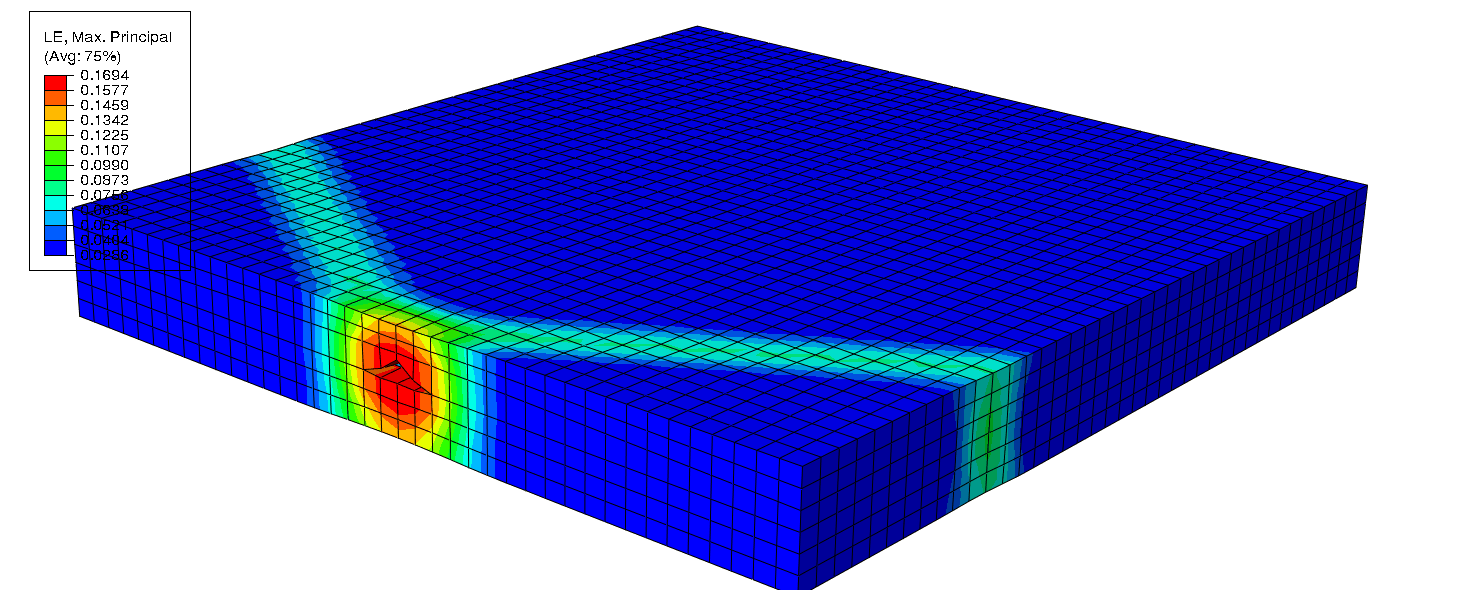
\includegraphics[width=\textwidth]{appendix_b/figures/0125p1.png}
    \caption{0.125 aspect ratio, 1 direction}
  \end{subfigure}
  \\
  \begin{subfigure}[b]{0.6\textwidth}
    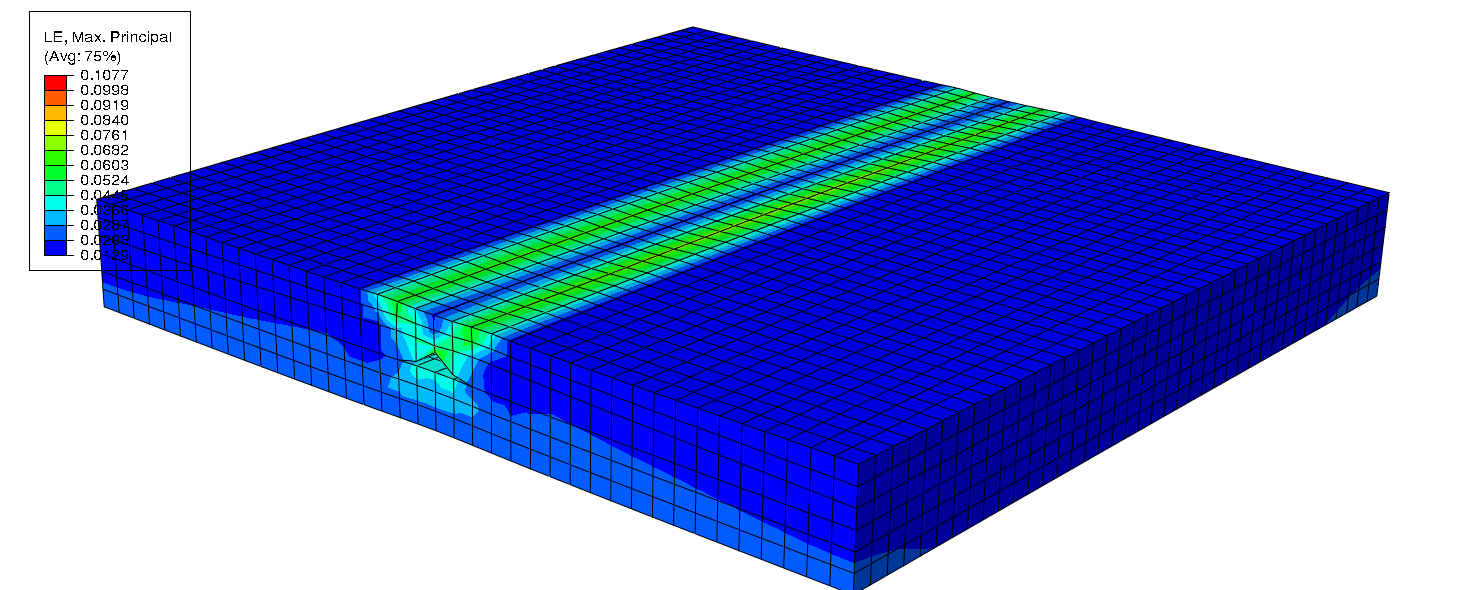
\includegraphics[width=\textwidth]{appendix_b/figures/0125p2.png}
    \caption{0.125 aspect ratio, 2 direction}
  \end{subfigure}
  \\
    \begin{subfigure}[b]{0.60\textwidth}
    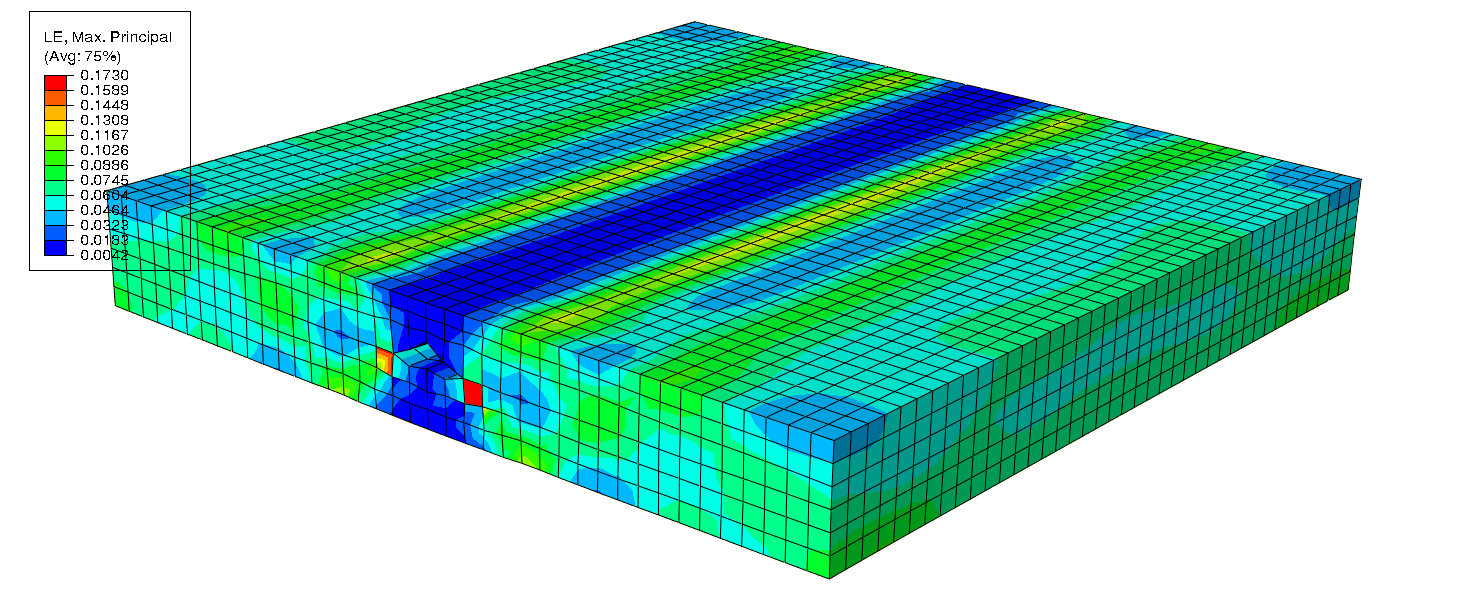
\includegraphics[width=\textwidth]{appendix_b/figures/0125p3.png}
    \caption{0.125 aspect ratio, 3 direction}
  \end{subfigure}
  \end{figure}
  
 \begin{figure}
   \begin{subfigure}[b]{0.70\textwidth}
    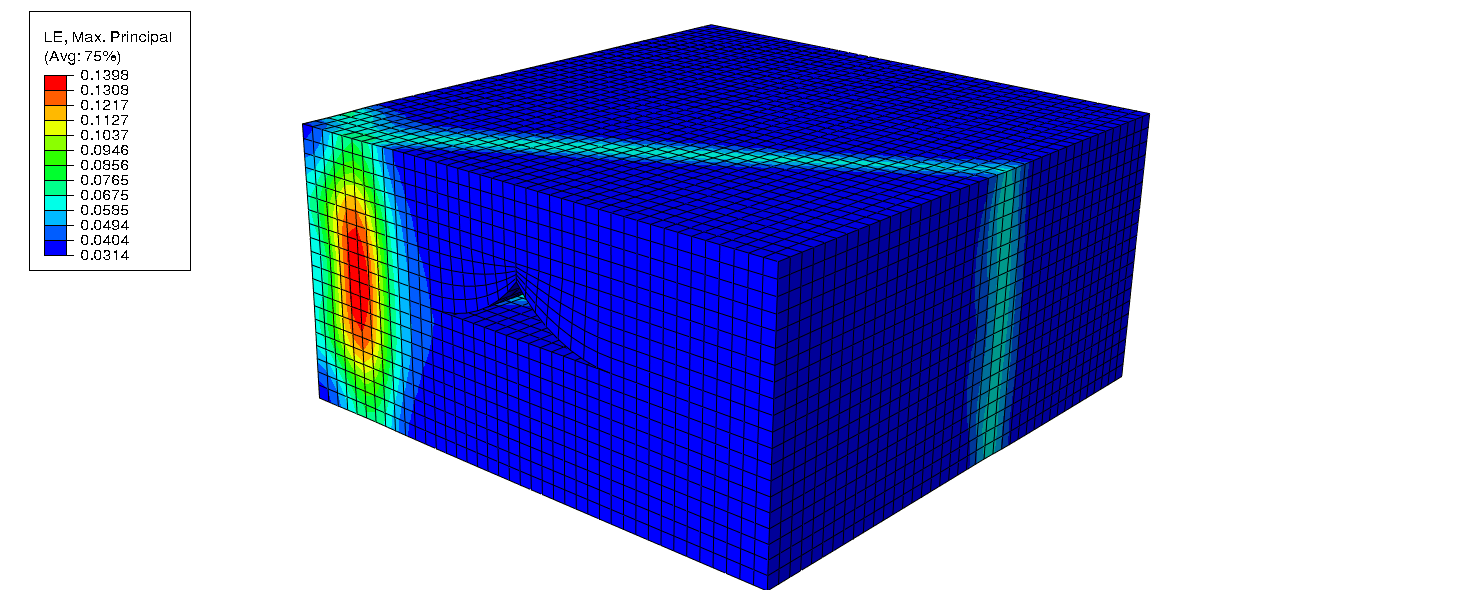
\includegraphics[width=\textwidth]{appendix_b/figures/05p1.png}
    \caption{0.5 aspect ratio, 1 direction}
  \end{subfigure}
  \\
    \begin{subfigure}[b]{0.70\textwidth}
    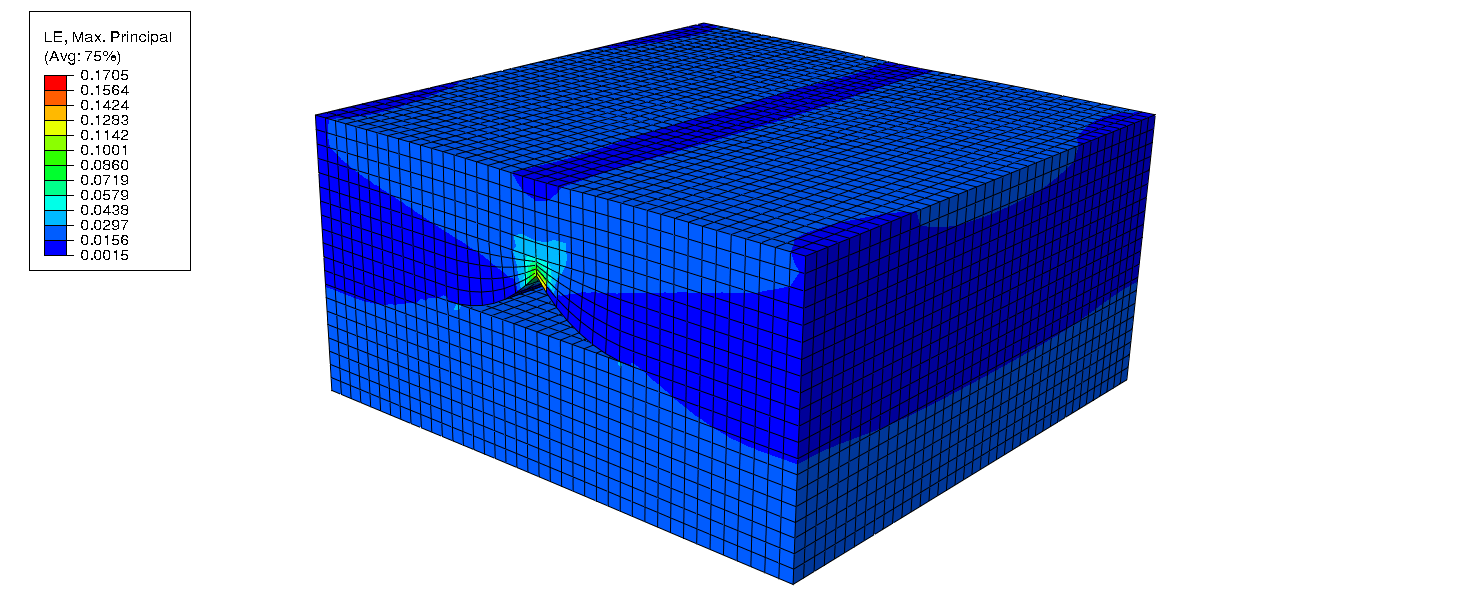
\includegraphics[width=\textwidth]{appendix_b/figures/05p2.png}
    \caption{0.5 aspect ratio, 2 direction}
  \end{subfigure}
  \\
  \begin{subfigure}[b]{0.70\textwidth}
    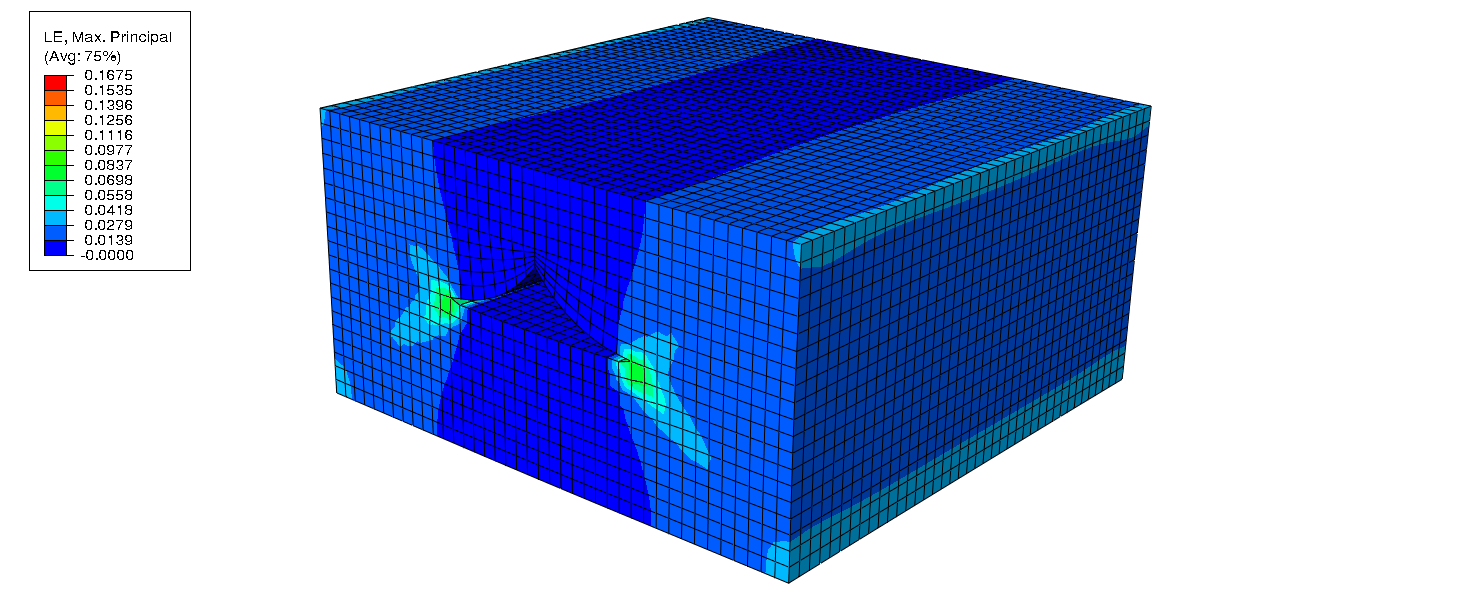
\includegraphics[width=\textwidth]{appendix_b/figures/05p3.png}
    \caption{0.5 aspect ratio, 3 direction}
  \end{subfigure}
\end{figure}
\\
\begin{figure}
    \begin{subfigure}[b]{0.80\textwidth}
    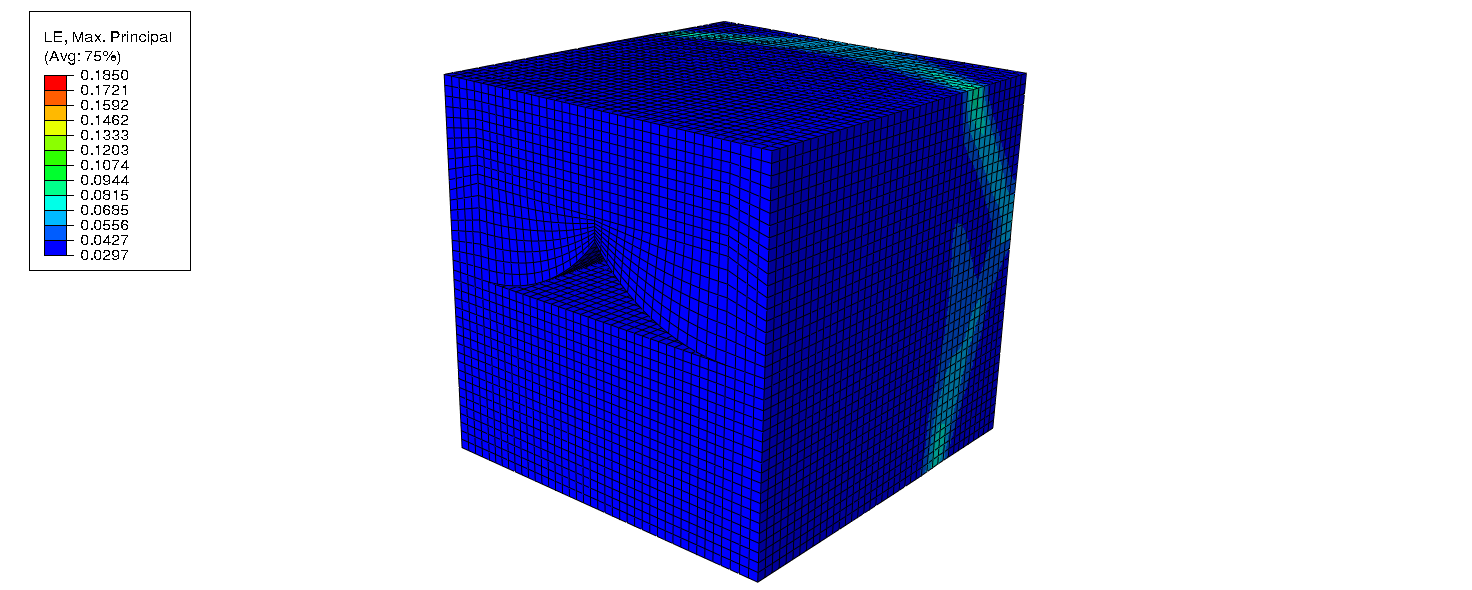
\includegraphics[width=\textwidth]{appendix_b/figures/1p1.png}
    \caption{1 aspect ratio, 1 direction}
  \end{subfigure}
  \\
    \begin{subfigure}[b]{0.80\textwidth}
    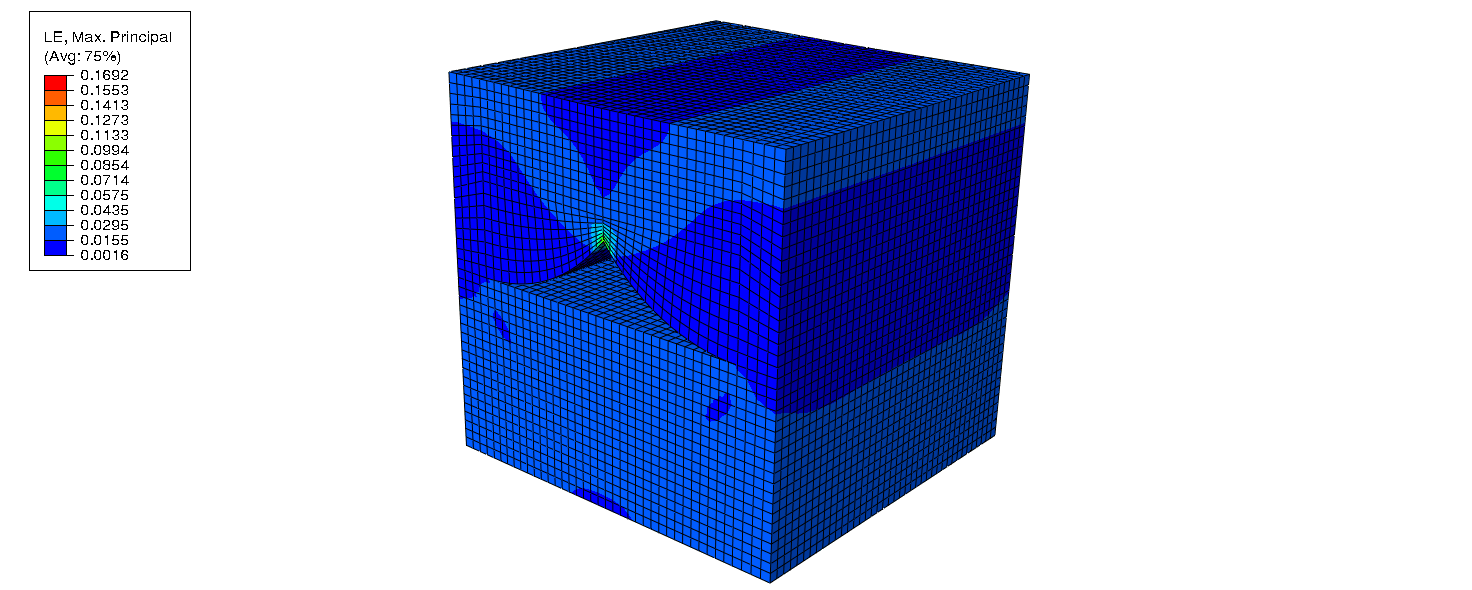
\includegraphics[width=\textwidth]{appendix_b/figures/1p2.png}
    \caption{1 aspect ratio, 2 direction}
  \end{subfigure}
  \\
  \begin{subfigure}[b]{0.80\textwidth}
    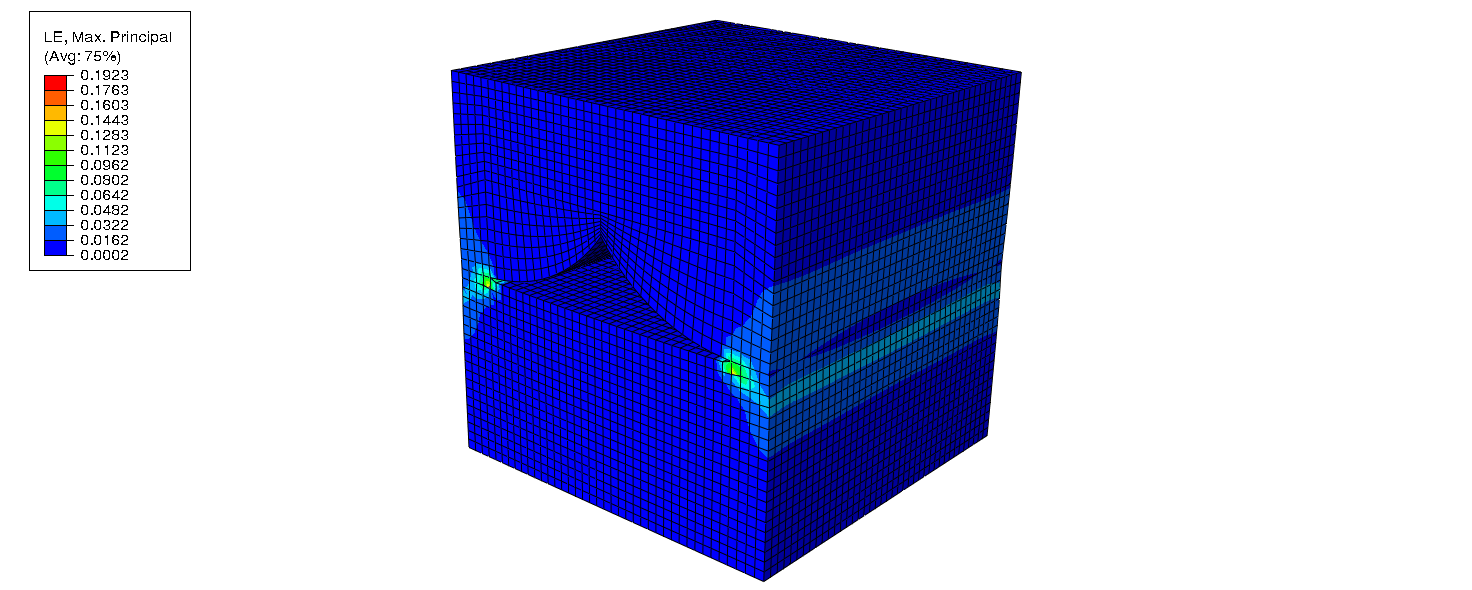
\includegraphics[width=\textwidth]{appendix_b/figures/1p3.png}
    \caption{1 aspect ratio, 3 direction}
  \end{subfigure}
  \caption{Contour plots for strain of different aspect ratios just before failure}
  \label{fig:Contourplot}
\end{figure}
\clearpage

\begin{figure}
\centering
  \begin{subfigure}[b]{1\textwidth}
    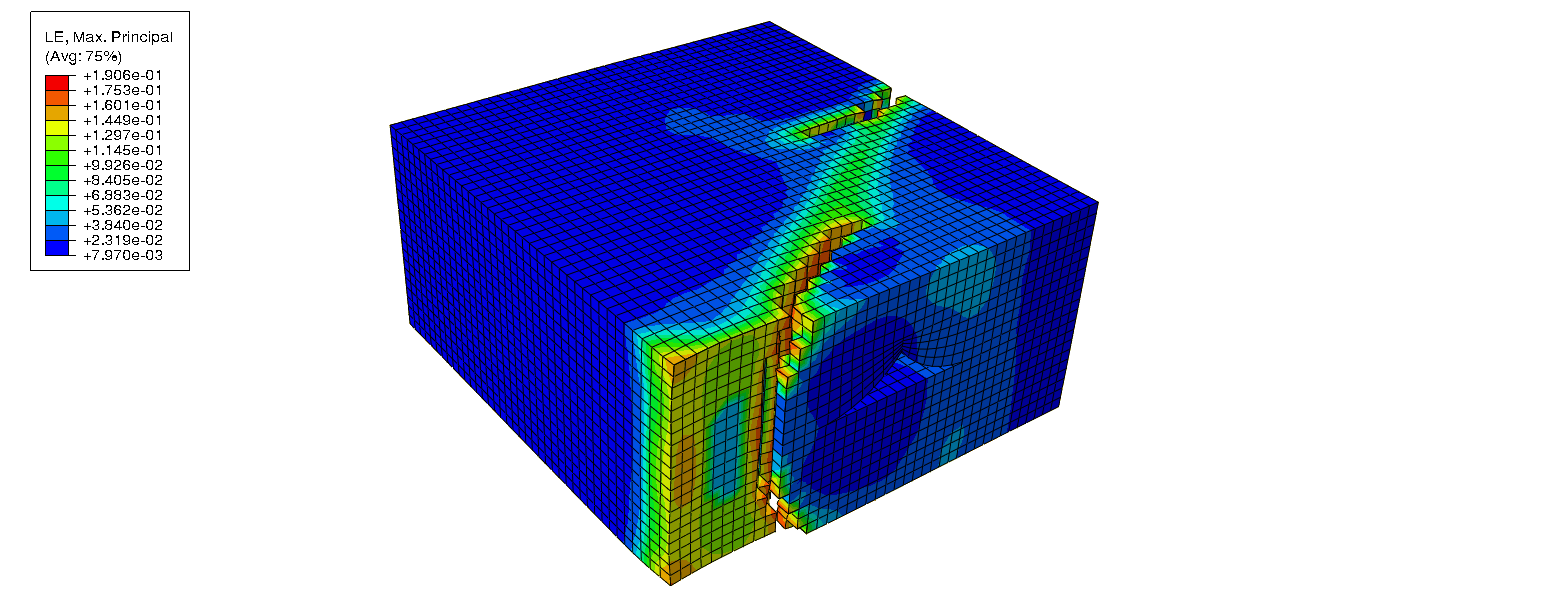
\includegraphics[width=\textwidth]{appendix_b/figures/p1_05crack.png}
    \caption{0.5 aspect ratio, loaded in 1 direction}
  \end{subfigure}
  \\
  \begin{subfigure}[b]{0.6\textwidth}
    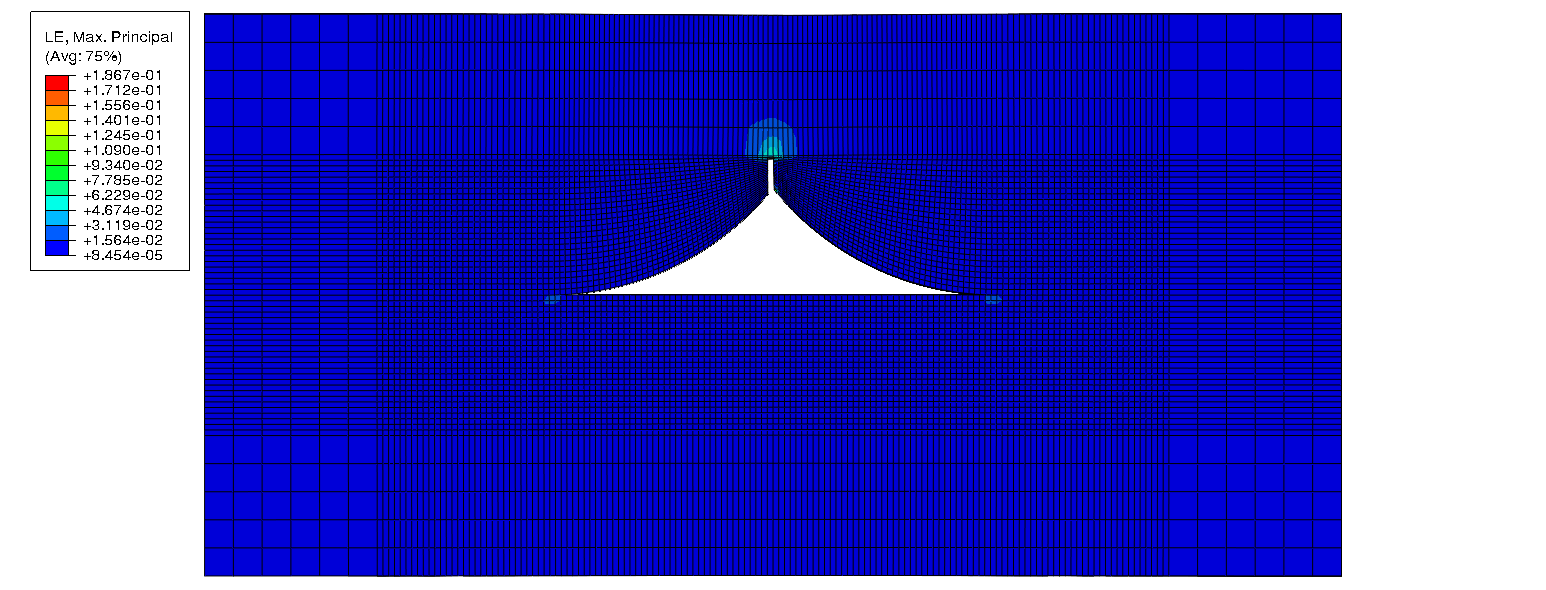
\includegraphics[width=\textwidth]{appendix_b/figures/p2_05crack.png}
    \caption{0.5 aspect ratio, loaded in 2 direction}
  \end{subfigure}
  \\
    \begin{subfigure}[b]{0.60\textwidth}
    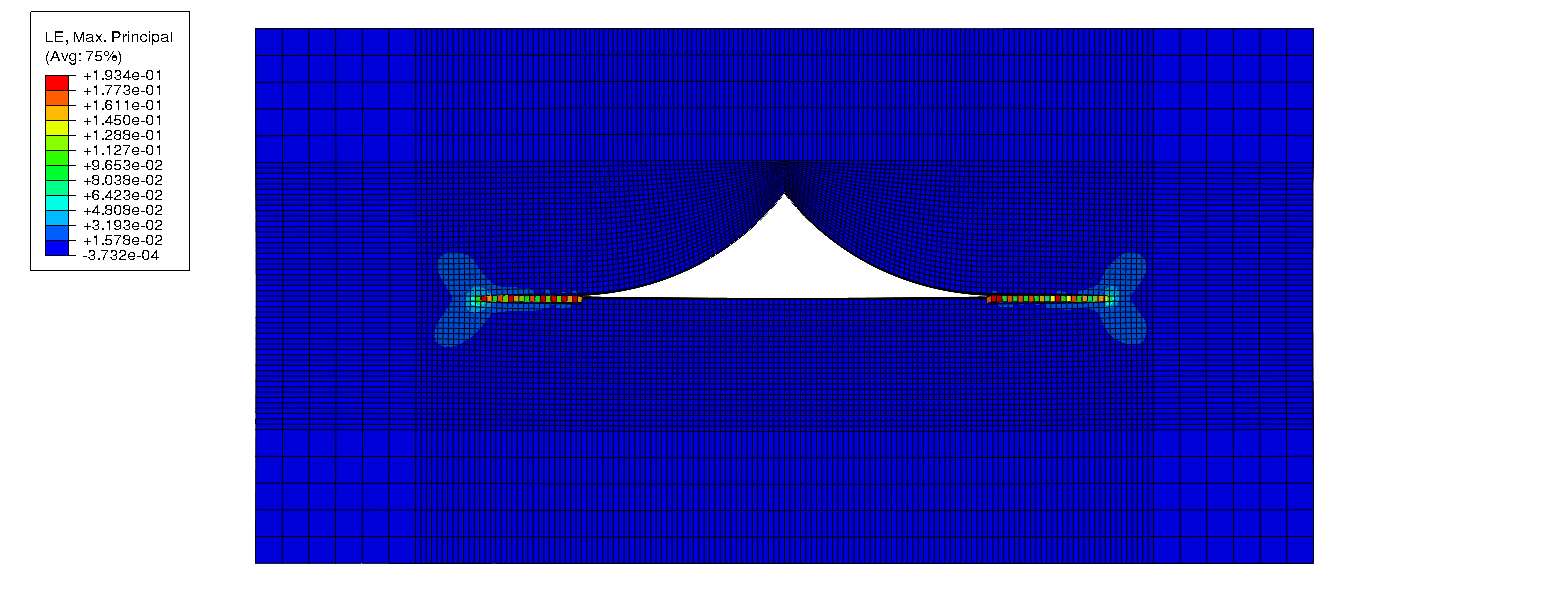
\includegraphics[width=\textwidth]{appendix_b/figures/p3_05crack.png}
    \caption{0.5 aspect ratio, loaded in 3 direction}
  \end{subfigure}
  \\
    \caption{Contour plots of equivalent strain for crack propagation of 0.5 aspect ratio}
  \label{fig:Contourplot}
  \end{figure}


%Some people like to have the references at the end of chapters, instead of at the end of the thesis. However, compiling the document becomes a little less convenient and I do not see the benefit of doing this. Anyway, in case you want to do that then you need to edit the \texttt{dissertation.cls} file by uncommenting the \texttt{chapterbib} package and including \texttt{sectionbib} in the \texttt{natbib} package. Then, you have to include the special command \texttt{\textbackslash references\{references\}} at the end of \textbf{each} chapter (for example, at the end of \texttt{chapter\_1.tex}). Note that the references are included in the file \texttt{references.bib}.

%Also note that if you want to have references at the end of chapters you need to run a command like \texttt{bibtex chapter\_1/chapter\_1} for each chapter. For convenience, a ``Makefile'' is also available (although you need to edit it), so you can run this file and compile the entire document such that references are put at the end of each chapter. Again, my recommendation is to just ignore this completely, and use the standard format of references at the end of the thesis. 